\documentclass[a4paper]{article}

\usepackage[utf8]{inputenc}
\usepackage[portuges]{babel}
\usepackage{a4wide}
\usepackage{graphicx}
\usepackage{underscore}


\title{Projeto de Laboratórios de Informática 3\\Grupo 20}
\author{Diogo Miguel Alves Rocha (A79751) \and Gabriela Sá Martins (A81987) \and Ricardo Milhazes Veloso (A81919) \and Ricardo Jorge Silva Ferreira (82568)}
\date{\today}

\begin{document}

\maketitle

\begin{abstract}

O objetivo deste trabalho consistiu em criar um programa que permitisse a extração e análise de dados provenientes da base de dados correspondente ao StackOverFlow. Tendo como objetivo final a resposta a um determinado número de querys , em que o tempo de execução será o mais reduzido possível.

\end{abstract}

\tableofcontents

\section{Introdução}
\label{sec:intro}
O trabalho proposto tinha em vista a resolução de 11 interrogações da forma mais eficiente e rápida possível. Para que conseguissemos corresponder a estas medidas criamos quatro estruturas, todas elas HashTables .


\section{Descrição do Problema}

O principal problema era criar uma estrutura capaz de armazenar todos os dados provenientes da base de dados correspondente ao StackOverFlow, de maneira que o acesso a esses mesmos dados fosse o mais rápido possível que por consequência a resposta às interrogações fosse ainda mais rápida, e sem memory leaks.

\section{Concepção da Solução}

Com vista a resolver o problema decidimos criar 4 HashTables, uma com os dados do utilizador,\textbf{h_IDUtilizador},outra com os dados referentes aos posts do tipo pergunta \textbf{h_IDPerguntas},outra com os dados referentes aos posts do tipo resposta \textbf{h_IDRespostas}, e por fim outra com as tags \textbf{h_IDTags}. Cada uma das anteriores será explicitada numa secção posterior referente às mesmas. 

	\subsection{Porquê da HashTable}

O principal motivo da escolha deste tipo de estrutura de dados foi o tempo de procura de um elemento que no melhor caso vai ser sempre constante e é o tipo de estrutura que apresenta o tempo de procura inferior em relação a outros.

 
\begin{figure}[ht]
\centering
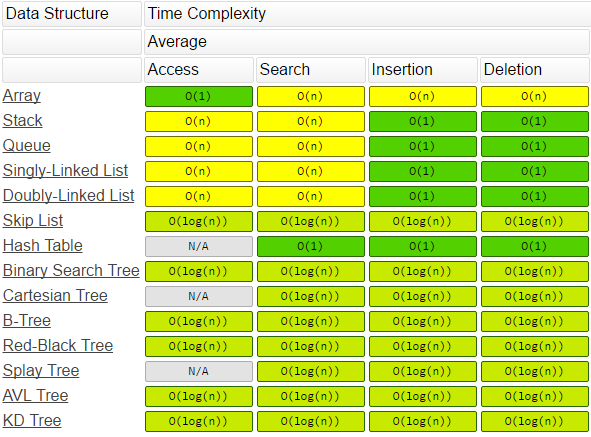
\includegraphics[scale =0.25]{timecomplexity.jpeg}
\caption{timecomplexity}
\label{img:time_complexity}
\end{figure}


\section{A Estrutura}

\begin{figure}[ht]
\centering
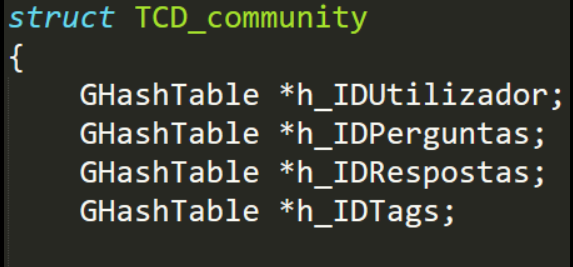
\includegraphics[scale =0.25]{tcd.png}
\caption{TCD_community}
\label{img:tcd}
\end{figure}

	\subsection{h_IDUtilizador}
	A estrutura contém informações relativas ao \textbf{utilizador}, e apresenta 7 parâmetros diferentes:

	\begin{description}
		\item[id_u] -ID do utilizador;
		\item[name] -Nome do utilizador;
		\item[shortb] -Short bio do utilizador;
		\item[totalposts] -Número total de posts;
		\item[reputacao] -Reputação do utilizador;
		\item[votes] -Número de votes do utilizador;
	\end{description}
	

	\begin{figure}[ht]
	\centering
	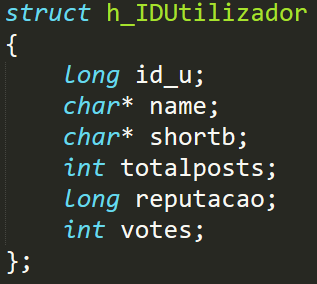
\includegraphics[scale =0.25]{utilizador.png}
	\caption{h_IDUtilizador}
	\label{img:h_IDUtilizador}
	\end{figure}

	\subsection{h_IDPerguntas}
	A estrutura contém informações relativas às \textbf{Perguntas}, e apresenta 7 parâmetros diferentes:

	\begin{description}
		\item[id_post] -ID da pergunta;
		\item[id_autor] -ID do autor da pergunta;
		\item[title] -Título da pergunta;
		\item[tags] -Tag da pergunta;
		\item[reputacao] -Reputação do utilizador;
		\item[n_resp] -Número de respostas àquela pergunta;
		\item[d] -Data da pergunta;
	\end{description}


	\begin{figure}[ht]
	\centering
	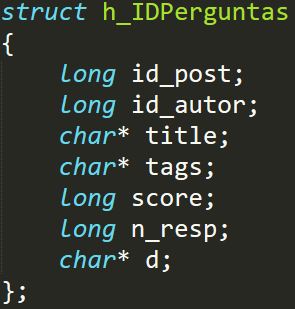
\includegraphics[scale =0.25]{perguntas.png}
	\caption{h_IDPerguntas}
	\label{img:h_IDPerguntas}
	\end{figure}

	\subsection{h_IDRespostas}
	A estrutura contém informações relativas às \textbf{Respostas}, e apresenta 6 parâmetros diferentes:

	\begin{description}
		\item[id_post] -ID da Resposta;
		\item[id_perg] -ID da pergunta correspondente à resposta;
		\item[id_autor] -ID do autor da resposta;
		\item[score] -Score da resposta;
		\item[n_coments] -Número de comentários aquela resposta;
		\item[d] -Data da Resposta;

	\end{description}


	

	\begin{figure}[ht]
	\centering
	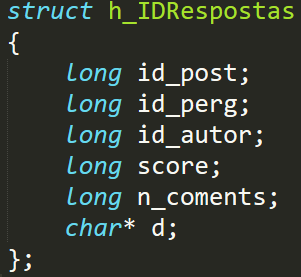
\includegraphics[scale =0.25]{respostas.png}
	\caption{h_IDRespostas}
	\label{img:h_IDRespostas}
	\end{figure}

	\subsection{h_IDTags}
	A estrutura contém informações relativas às \textbf{Tags}, e apresenta 3 parâmetros diferentes:

	\begin{description}
		\item[id_tag] -ID da tag;
		\item[tag] -Tag;
		\item[count] -Conta o número de vezes que uma Tag é utilizada num intervalo de tempo;
	\end{description}	


	\begin{figure}[ht]
	\centering
	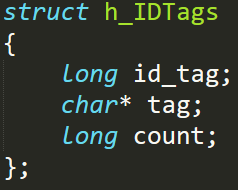
\includegraphics[scale =0.25]{tags.png}
	\caption{h_IDTags}
	\label{img:h_IDTags}
	\end{figure}

	

\section {Extração de Informação}

	\subsection{Pergunta 1}
	Na pergunta 1 temos de retornar um par com o titulo do posto correspondente ao id recebido, e com o nome do utilizador a que esse post pertence. A função utilizada é a \textbf{g_hash_table_lookup.}

	\subsection{Perguntas 2,3,4,5,6,7,8,9,10,11}
	As seguintes perguntas foram obtidas usando a mesma função \textbf{getNextIterator}.

		\subsubsection{Pergunta 2}
			Nesta pergunta queremos saber o Top N utilizadores com maior número de posts e para isso consultamos a variável totalposts.
		\subsubsection{Pergunta 3}
		Nesta pergunta queremos obter o número total de posts num determinado periodo de tempo mas com perguntas e respostas em separado. Para isso depois de consultar a data em cada uma das hashatbles e comparar com a que é estipulada consultamos a variável id_post tanto na hashtable de perguntas como a de respostas. Returnado um par com o respetivo número de perguntas e respostas total.

		\subsubsection{Pergunta 4}
		Nesta pergunta queremos obter o número total de perguntas contendo uma determinada tag num determinado periodo de tempo, e retornar essas perguntas por cronologia inversa.
		Para isso depois de consultar a data em cada uma das hashatbles e comparar com a que é estipulada consultamos a variável tags , e retornamos uma lista com o id dessas mesmas tags. 
		\subsubsection{Pergunta 5}
		 Nesta pergunta queremos devolver a informação do
		perfil do utilizador (short bio) e os IDs dos seus 10 últimos posts (perguntas ou respostas),ordenados por cronologia inversa. Para isso devolvemos uma struct userinfo que contém a variável short_bio e ultimos10;
		\subsubsection{Pergunta 6}
		Nesta pergunta queremos saber, num intervalo de tempo arbitrario, quais as N respostas com mais votos, devolvendo uma lista com  a variável id_post.
		\subsubsection{Pergunta 7}
		Nesta pergunta o objetivo é dado um intervalo de tempo arbitrário devolver os id's das N perguntas com mais respostas. Por ordem decrescente do número de respostas.
		Devolvendo uma lista com o Top N das variaveis Id_post.
		\subsubsection{Pergunta 8}
		Nesta pergunta o objetivo é dado uma palavra, devolver uma lista com os id's de n perguntas cujos titulos a contenham, ordenados por cronologia inversa. para responder utilizamos a variável id_post, devolvendo uma lista destas.
		\subsubsection{Pergunta 9}
		Nesta pergunta recebendo o ID de dois utilizadores devolver as últimas N perguntas que em que participaram esses dois utilizadores.
		Para isso é devolvida uma lista com a variável ultimasN;
		\subsubsection{Pergunta 10}
		Nesta pergunta recebendo o ID de uma pergunta obter a melhor resposta. Para isso retornamos a variável id_melhor.
		\subsubsection{Pergunta 11}
		Nesta pergunta recebendo um intervalo de tempo arbitrário devolver os ids das N tags mais usadas peços N utilizadores com maior reputação. Para isso retornamos uma lisata com a variável user_best_rep;

		
\section {Resultados}

\begin{figure}[ht]
	\centering
	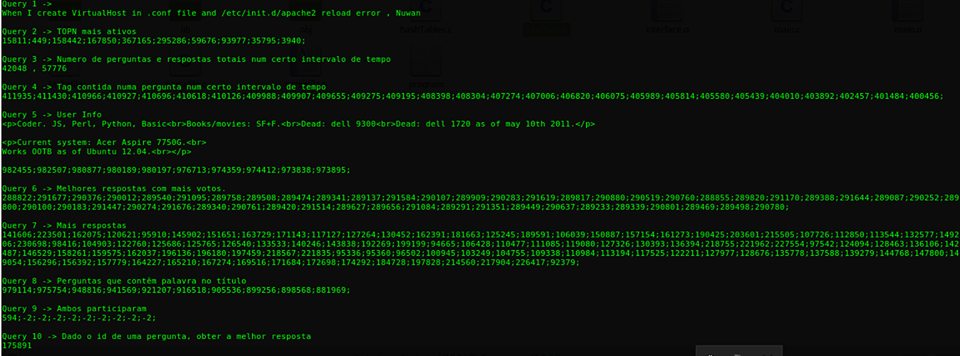
\includegraphics[scale =0.50]{resultados.png}
	\caption{Resultados}
	\label{img:Resultados}
	\end{figure}

\section {Teste de Tempo}

\begin{figure}[ht]
	\centering
	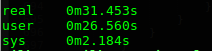
\includegraphics[scale =0.50]{tempo.png}
	\caption{tempo}
	\label{img:tempo}
	\end{figure}

\section {Memory Leaks}

\begin{figure}[ht]
\centering
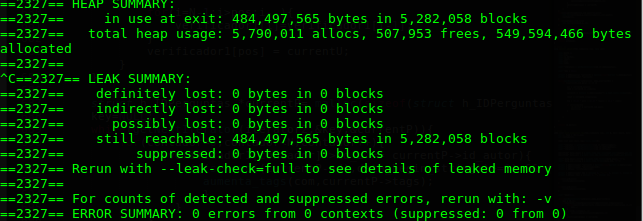
\includegraphics[scale =0.50]{leaks.png}
\caption{leaks utilizando o programa Valgrind}
\label{img:leaks}
\end{figure}





\section{Conclusão}
Em suma todos os objetivos propostos foram atingidos. Toda a extração de informação proveniente da base de dados do site \textbf{StackOverflow} e análise da mesma é feita de uma maneira eficiente, com um tempo de execução bastante aceitável e sem qualquer perda de informação. 


\end{document}